\problemname{Gnoll Hypothesis}

You are a huge fan of the RPG \emph{The Eldest Scrolls: Earthrim} and know all of the game's internal mechanics.
For instance, when spawning a new monster, each of the $n$ different types of monsters in the game has some fixed probability of appearing,
and you know exactly what this probability distribution over monster types is.

However, in the latest update the developers seem to have changed the way monsters are spawned.  After some testing and reverse engineering,
you realise that instead of spawning all $n$ types of monsters, each spawn location only has a spawn pool of $k$ monster types. These spawn pools are
chosen randomly at the start of the game, independently for each spawn location, with every monster type having the same chance of being chosen for the spawn pool.  And apparently
a developer was lazy with adjusting the spawn chances.  Instead of normalising the spawn chances of the $k$ chosen types, the developer decided that
if a type of monster is not chosen, its spawn chance is added to the next chosen monster type in the list of types (and if monster types at the end of the list are not
chosen, their spawn chances are added to the first chosen monster type in the list).  For example, Figure~\ref{spawning monsters sample 1} shows a small example with $n=5$ monsters, a possible random choice of $k=3$ of those monsters, and the resulting spawn probabilities for those $3$ monsters.

After the update, some monster types seem to appear less often than before, and
some more often (for instance now there seem to be Gnolls all over
the place).  You believe that the new spawning logic may be
responsible for this by having changed the effective spawn chances of
the monsters.  In order to test this hypothesis, you decide to compute
these effective spawn chances after the update.

\begin{figure}[h] \centering
  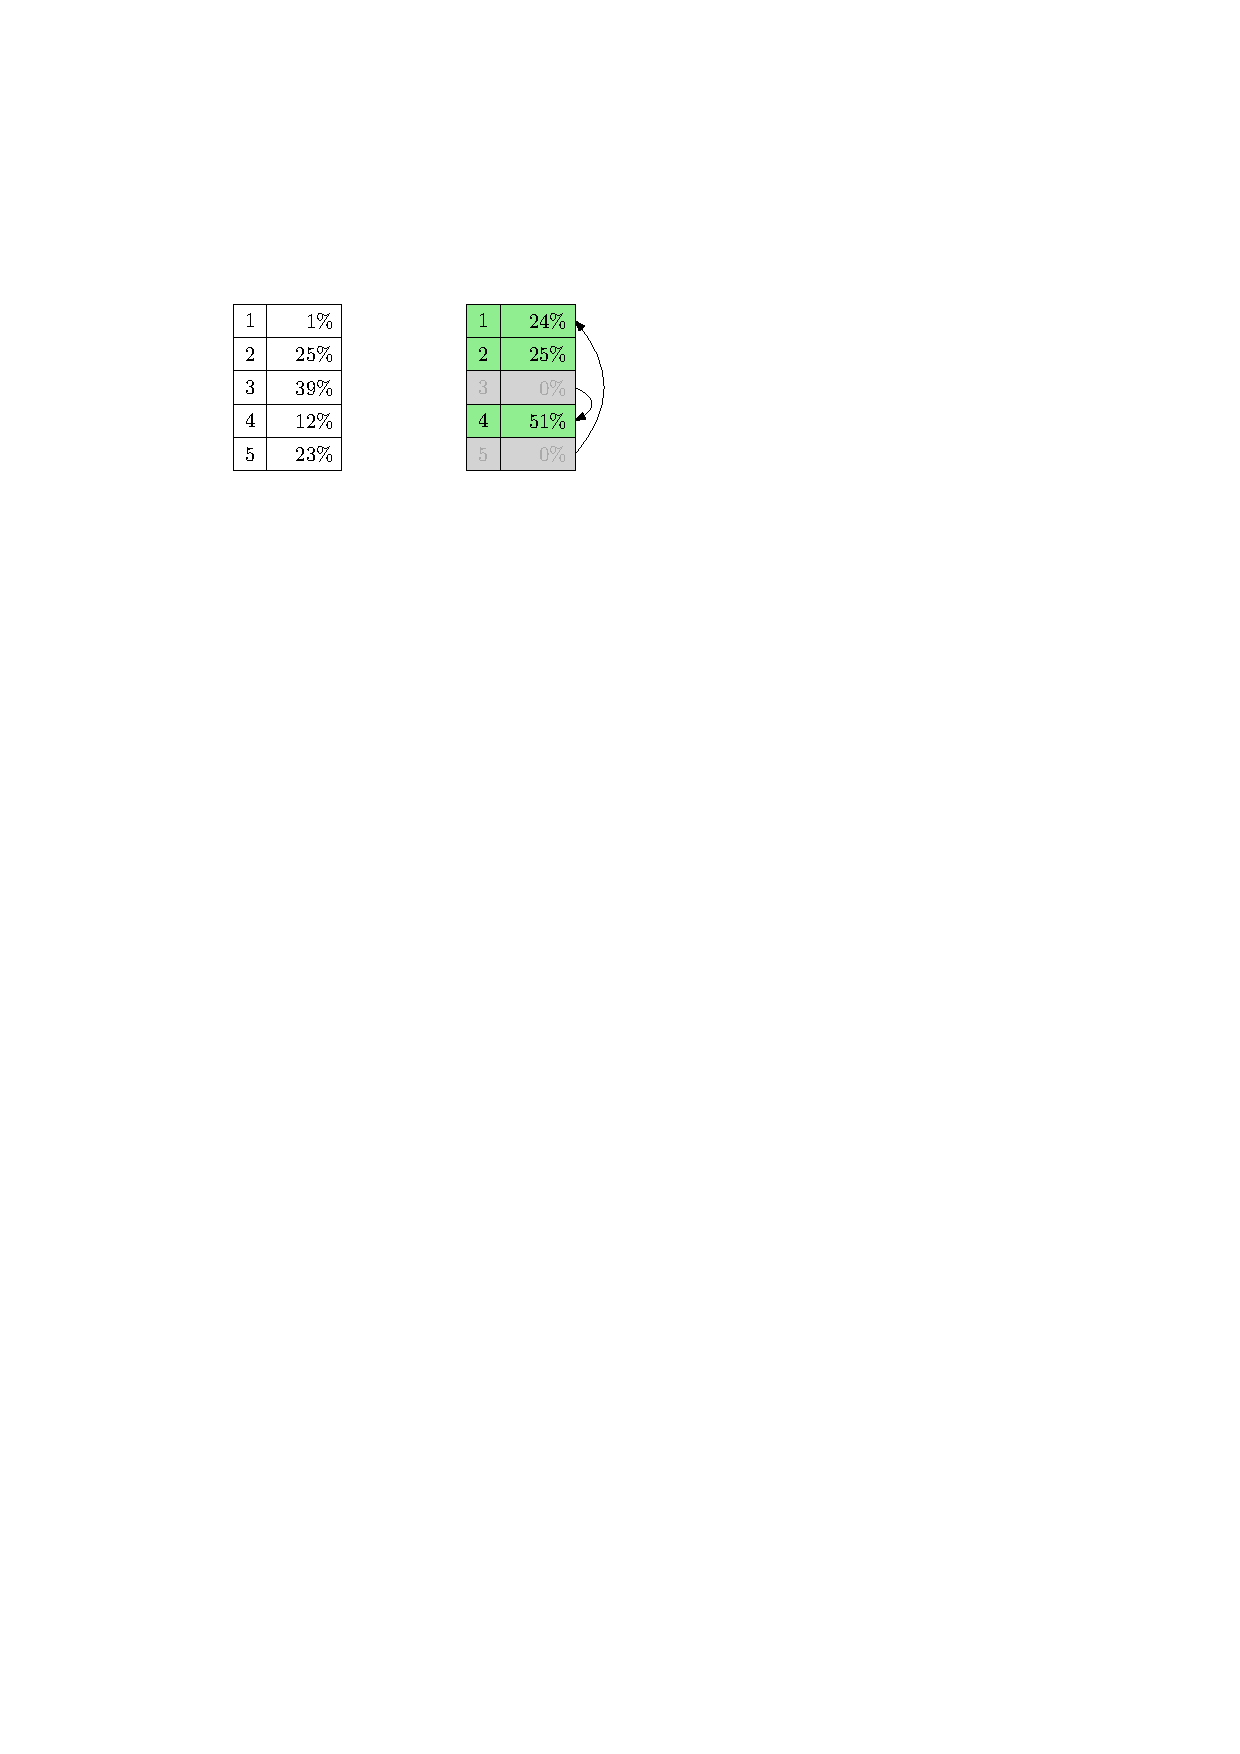
\includegraphics[width=.4\textwidth]{sample1}
  \caption{Sample Input 1 and one possible spawn pool with adjusted spawn chances.}
  \label{spawning monsters sample 1}
\end{figure}

\section*{Input}
The input consists of:
\begin{itemize}
  \item One line with two integers $n$ and $k$ ($1 \le k \le n \le 500$), the number of different types of monsters and the number of monsters that are randomly chosen
    for the spawn pool of each spawn location.
  \item One line with $n$ real numbers $s_1, s_2, \ldots, s_n$ ($s_i \ge 0$ for each $i$, $\sum^{n}_{j=1}s_j = 100$), where $s_i$ is the spawn chance in percent for the $i$th type in the list of monster types.  Every real number has at most six digits after the decimal point.
\end{itemize}

\section*{Output}
Output a single line containing $n$ real numbers, the effective spawn chance in percent of each type of monster. The $i$th number in your output should correspond to the $i$th type of monster.
Your answers should have an absolute or relative error of at most $10^{-6}$.
